\documentclass[../EBEXPaper2.tex]{subfiles}
\begin{document}
%------------------------------------------------- 
\section{Focal Plane Layout}
\label{sec:focal_plane_layout}

\ac{EBEX} had two focal planes that were cooled to a bath temperature of $\sim$0.25~K. The cryogenic system is described in \ac{EP1}.
Each focal plane consisted of a layer of electromagnetic filters, a monolithic
array of feedhorns attached to a monolithic array of waveguides, 7 detector wafers, wafer holders 
and ``\ac{LC} Boards", 
and a back-cover which, together with the array of horns, completed a Faraday cage around 
the detectors; see Figure~\ref{fig:EBEX_Focal_Plane}. The electromagnetic filters and waveguides 
defined frequency bands centered on 150, 250, and 410~GHz. Each focal plane was arranged such that 
4 wafers operated at 150~GHz, 2 at 250~GHz, and 1 at 410~GHz. The \ac{LC} boards were part of the 
multiplexed frequency domain bias and readout of the detectors, see Section~\ref{sec:detector_readout}. 
Each detector wafer had 141 micro-fabricated lithographically bolometers, of which 128 
were biased and readout with 8 pairs of wires.  

\begin{figure}[ht]
\centering
\subfigure[Exploded Solidworks View]
{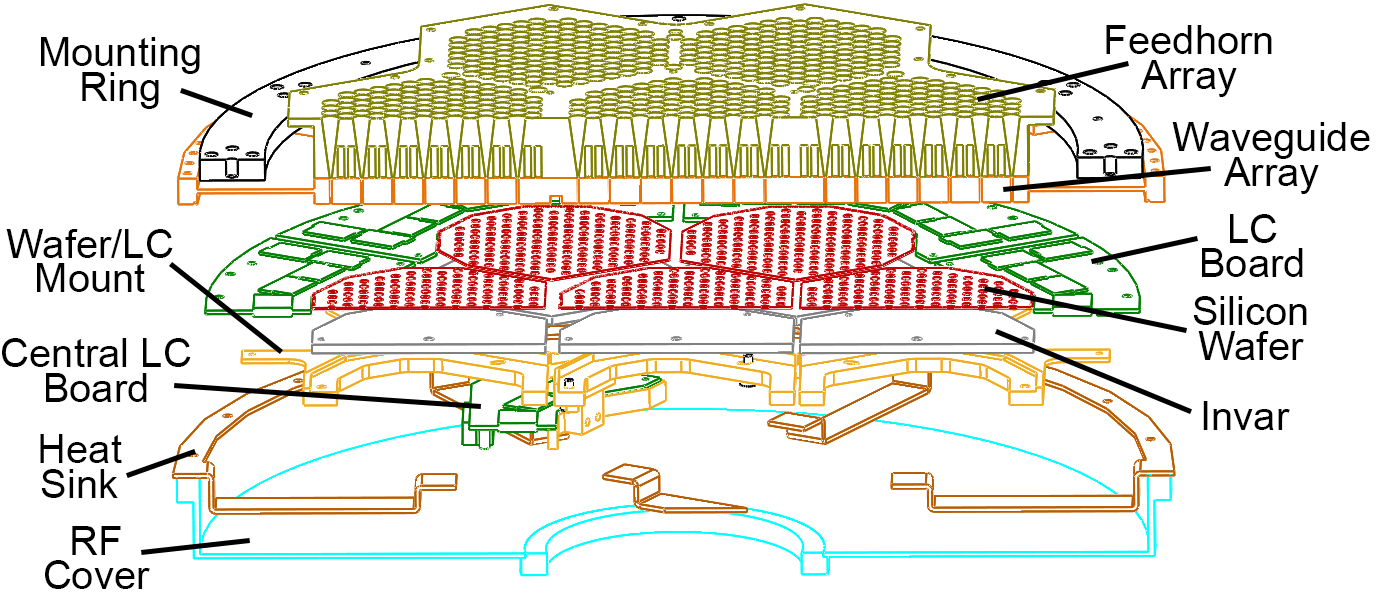
\includegraphics[width=0.6\textwidth]{./images/Focal_Plane_Zoom.png}}
\subfigure[Single Focal Plane Unit]
{\includegraphics[width=0.3\textwidth]{./images/EBEX_Focal_Plane_Photo_Annotated.pdf}}
\caption{\textbf{LEFT:} Solidworks rendering of the edge of a single wafer module demonstrating the integration scheme for \ac{EBEX}.  Each of the subcomponents is aligned with dowel pins and secured with screws.  Both of the focal plane units were assembled before being installed into the cryostat. \textbf{RIGHT:} A photograph of a single \ac{EBEX} focal plane with the central 410 GHz yet to be installed detailing the location of the 7 wafer in each focal plane and the supporting readout electronics. \label{fig:EBEX_Focal_Plane}}
\end{figure}

Each sub-array has niobium leads which provide electrical access from the bondpads at the edge of the wafer to the \ac{TES}s distributed across the wafer.   The niobium leads from all the detectors of a given wafer are channeled to wire bonding pads at the edge of the wafer and are bonded to pads at the edge of \ac{LC} boards, which contain inductors and capacitors that are part of the frequency domain multiplexing readout (see Section~\ref{sec:detector_readout}).  We place each silicon wafer onto a wafer-shaped piece of invar thinly coated with warmed Apiezon N grease. For the edge wafers, the invar is screwed into an aluminum mount holding the \ac{LC} board in the same plane as the wafer. The central wafer, however, is completely surrounded by other wafers, so its aluminum mount has standoffs to hold its \ac{LC} board in the plane just below the detectors. On either side of each wafer's aluminum mount, there are dowel pin holes to align it with the focal plane waveguide array. We place an alignment jig into the dowel pin holes and position the wafer such that the spider webs are visually aligned within holes positioned to account for thermal contraction. The assembly is shown on the left hand side of Figure \ref{fig:EBEX_Focal_Plane}.

We wirebond the silicon wafer's niobium bond pads directly to the copper bond pands on the \ac{LC} board. For the edge wafer \ac{LC} boards, the copper bond pads are on the G10 \ac{PCB}, while for the central \ac{LC} boards, the copper bond pads are on the ends of flexible Kapton strips extending from the offset G10 \ac{PCB} to aluminum blocks just next to the central wafer.

In series with each bolometer there is a single layer niobium lithographed 24 uH inductor chip, provided by NIST, and a stack of ceramic capacitors ranging from 900 to 30000 pF. The copper traces from a bundle of 16 detectors route to a single pair of copper wires within a Kapton strip and each Kapton strip has 8 pairs of wires. We connect the Kapton copper pigtail to the \ac{ELIS}s via a Micro-D connector.
\comred{BW: needs review by Kate/Kyle Z}

%------------------------------------------------
%\include{DetectorReadoutBibliography}
\end{document}  
